\documentclass[9pt,pdf,utf8,hyperref={unicode},aspectratio=169]{beamer}

%Привычный шрифт для математических формул
\usefonttheme[onlymath]{serif}
\mode<presentation>
{
    \usetheme{boxes}
    \beamertemplatenavigationsymbolsempty

    \setbeamercovered{transparent}
    \setbeamertemplate{navigation symbols}{}
    
    \setbeamertemplate{footline}[frame number]
    \setbeamertemplate{caption}[numbered]
    % \setbeamersize{text margin left=0.5em, text margin right=0.5em}
}

% Дополнительные библиотеки
\usepackage[T2A]{fontenc}
\usepackage[english, russian]{babel}
\usepackage[utf8]{inputenc}
\usepackage{amsmath,amssymb}
\usepackage{indentfirst}
\usepackage{changepage}
\usepackage{enumerate}
\usepackage{mathtools}
\usepackage{multicol}
\usepackage{multirow}
\usepackage{ragged2e}
\usepackage{multicol}
\usepackage{diagbox}
\usepackage{wrapfig}
\usepackage{comment}
\usepackage{subfig}
\usepackage{array}
\usepackage{color}
\usepackage{tikz}
\usepackage{url}
\usepackage{bm}

\usetikzlibrary{trees}

% Определение дополнительных функций
\DeclareMathOperator*{\plim}{\mathop{plim}}
\DeclareMathOperator{\prob}{\mathbf{P}\!}
\DeclareMathOperator{\arctanh}{arctanh}
\DeclareMathOperator{\mmode}{mode}
\DeclareMathOperator{\rank}{rank}
\DeclareMathOperator{\diag}{diag}
\DeclareMathOperator{\sign}{sign}
\DeclareMathOperator{\cov}{cov}
\DeclareMathOperator{\pow}{pow}
\DeclareMathOperator{\med}{med}

\def\argmin#1{ \mathop{\text{argmin}}\limits_{#1} }
\def\argmax#1{ \mathop{\text{argmax}}\limits_{#1} }

\renewcommand{\leq}{\leqslant}
\renewcommand{\geq}{\geqslant}

\DeclareMathOperator{\FWER}{FWER}
\DeclareMathOperator{\FDR}{FDR}
\newtheorem{Th}{Теорема}
\newtheorem{Def}{Определение}

% Основная часть

\title[Дисперсионный анализ ]{Прикладной статистический анализ данных\\ Дисперсионный анализ}
\author{Андрей Грабовой}
\date{}

\begin{document}
\tikzstyle{every node}=[draw=black,thick,anchor=west]
\tikzstyle{selected}=[draw=red,fill=red!30]
\tikzstyle{optional}=[dashed,fill=gray!50]

\begin{frame}
    \titlepage
\end{frame}

\begin{frame}
   \only<1>{
    \begin{block}{Пример, Bonnini, табл. 3.2} Исследуется эффективность четырёх жаропонижающих средств, в составе которых один и тот же активный ингридиент присутствует в разных дозировках. Для каждой из четырёх групп из 15~морских свинок известно изменение температуры после введения жаропонижающего. Есть ли различия в действии препаратов?
    \end{block}

}


   \only<2>{
    \begin{block}{Пример, Bonnini, табл. 3.2} Исследуется эффективность четырёх жаропонижающих средств, в составе которых один и тот же активный ингридиент присутствует в разных дозировках. Для каждой из четырёх групп из 15~морских свинок известно изменение температуры после введения жаропонижающего. Есть ли различия в действии препаратов?
    \end{block}
    \textbf{Наивная идея:}\\
    \begin{enumerate}
    \item воспользоваться двувыборочным критерием, сравнив все пары групп;
    \item сделать поправку на множественность гипотез;
    \item выбрать пары с наиболее значимыми отличиями.
    
    \end{enumerate}
}


   \only<3>{
    \begin{block}{Пример, Bonnini, табл. 3.2} Исследуется эффективность четырёх жаропонижающих средств, в составе которых один и тот же активный ингридиент присутствует в разных дозировках. Для каждой из четырёх групп из 15~морских свинок известно изменение температуры после введения жаропонижающего. Есть ли различия в действии препаратов?
    \end{block}
    \textbf{Наивная идея:}\\
    \begin{enumerate}
    \item воспользоваться двувыборочным критерием, сравнив все пары групп;
    \item сделать поправку на множественность гипотез;
    \item выбрать пары с наиболее значимыми отличиями.
    
    \end{enumerate}
    \textbf{Проблема: } решается более частная задача. Неясно как определять размер эффекта для всех групп в совокупности.
    
}

\end{frame}


\begin{frame}{Разновидности дисперсионного анализа (ANOVA)}
    \begin{itemize}
    \item по числу факторов: однофакторный (one-way), двухфакторный (two-way) и т.\,д
    \item по типу выборок: независимые (between-subjects), связанные (within-subjects, repeated measurements)
    \item по типу альтернативы: общая, тренда
    \item по типу эффектов: случайные (random-effects), фиксированные (fixed-effects)
    \item по типу уровней факторов: независимые, вложенные (nested), с~болтающимся контролем (dangling control group), латинский квадрат (latin square)
	\item по используемым предположениям: нормальный, непараметрический 
	\item по объёму выборок: одинаковый (balanced), различный (unbalanced)
    \end{itemize}
\end{frame}


\section{1-way b.s.}
\subsection{Омнибус-критерии}
\begin{frame}{Однофакторный дисперсионный анализ}
    \only<1>{
    Пусть имеется $K$ выборок:
    $$X^N = X_1^{n_1}\bigcup X_2^{n_2}\bigcup\ldots\bigcup X_K^{n_K}, \;\; N = \sum\limits_{i=1}^K n_i.$$

    \bigskip

    Эквивалентная запись в виде псевдотаблицы:

    фактор $f\colon X \rightarrow \left\{1,\ldots,K\right\}$

    \bigskip

    \begin{center}
        \begin{tabular}{|c|c|c|c|c|c|} \hline
        $f$   & $1$ & $\ldots$ & $k$ & $\ldots$ & $K$ \\ \hline
        $X^N$ & $\footnotesize{\begin{matrix} X_{11} \\ \vdots \\ X_{1n_{1}} \end{matrix}}$ & \ldots & $\footnotesize{\begin{matrix} X_{k1} \\ \vdots \\ X_{kn_{k}} \end{matrix}}$ & \ldots & $\footnotesize{\begin{matrix} X_{K1} \\ \vdots \\ X_{Kn_{K}} \end{matrix}}$    \\\hline
        \end{tabular}
    \end{center}

    \bigskip

    \textbf{Задача}: проверить гипотезу об отсутствии влияния фактора $f$ на среднее значение признака $X$, то есть, о равенстве средних значений $K$ выборок.
    }

    \only<2>{
    \textbf{Идея}: рассмотрим две компоненты разброса значений $X_{ki}$ относительно глобального среднего $\bar{X}$:
    $$X_{ki}-\bar{X} = \left(X_{ki} - \bar{X}_k\right) + \left(\bar{X}_k - \bar{X}\right),$$
    где $\bar{X}_k$~--- среднее в $k$-й выборке.

    \bigskip

    Возведём в квадрат и просуммируем:
    \begin{align*}
        \sum_{k=1}^K \sum_{i=1}^{n_k} \left(X_{ki}-\bar{X}\right)^2 & = \sum_{k=1}^K \sum_{i=1}^{n_k} \left(X_{ki} - \bar{X}_k\right)^2 + \sum_{k=1}^K n_k\left(\bar{X}_k - \bar{X}\right)^2, \\
        SS_{total} & = SS_{wg} + SS_{bg}.
    \end{align*}

    Если средние в группах значительно отличаются, преобладает вторая компонента, если же они одинаковы~--- первая.
    }
    
    \only<3>{
    Линейная модель:
    $$X_{ki} = \mu + \alpha_k + \varepsilon_{ki},$$
    $i=1,\dots,n_k, \; k=1,\dots,K.$

    \bigskip

    $\mu$~--- глобальное среднее значение признака $X$,

    $\alpha_k$~--- отклонение от $\mu$, вызванное влиянием $k$-го уровня фактора $f$,

    $\varepsilon_{ki}$~--- случайные независимые одинаково распределённые ошибки.

    \bigskip

    Средние значения $X$ во всех $K$ выборках одинаковы $\Leftrightarrow$ $\alpha_1=\dots=\alpha_K$.    
    }
\end{frame}


\begin{frame}{Распределение Фишера}
%%%%%%%%%%%%%%%%%%%%%%%%%%%%%%%%%%%%%%%%%%%%%%%%%%%%%%%%%%%%%%%%%%%%%%%
% Распределение Фишера может выглядеть очень по-разному при разных значениях своих параметров.
%%%%%%%%%%%%%%%%%%%%%%%%%%%%%%%%%%%%%%%%%%%%%%%%%%%%%%%%%%%%%%%%%%%%%%%

    \only<1>{
    \begin{itemize}
    \item пусть $X_1\sim\chi^2_{d_1},$\; $X_2\sim\chi^2_{d_2},$  \; $X_1$ и $X_2$ независимы, тогда
    $$\frac{X_1/d_1}{X_2/d_2} \sim F\left(d_1,d_2\right)$$
    \item  если $X\sim F\left(d_1,d_2\right),$ то
    $$Y = \lim_{d_2\rightarrow \infty} d_1X \sim \chi^2_{d_1}$$
    \item $F\left(x,d_1,d_2\right) = F\left(1/x,d_2,d_1\right)$
    \item возникает в дисперсионном и регрессионном анализе
    \end{itemize}
    }

    

\end{frame}


\begin{frame}{Критерий Фишера}
    \only<1>{
    \begin{center}
        \begin{tabular}{rl}
            выборки:                        & $X^N = X_1^{n_1}\bigcup\ldots\bigcup X_K^{n_K}$ \\
            нулевая гипотеза:               & $H_0\colon \alpha_1=\dots=\alpha_K$ \\
            альтернатива:                   & $H_1\colon H_0$ неверна\\
            статистика:                     & $F\left(X^N\right) = \frac{SS_{bg} / \left(K-1\right)}{SS_{wg} / \left(N-K\right)}$ \\
                                            & $SS_{bg} = \sum\limits_{k=1}^K n_k\left(\bar{X}_k - \bar{X}\right)^2$ \\
                                            & $SS_{wg} = \sum\limits_{k=1}^K \sum\limits_{i=1}^{n_k} \left(X_{ki} - \bar{X}_k\right)^2$ \\
            нулевое распределение:          & $F(K-1, N-K)$\\
        \end{tabular}
        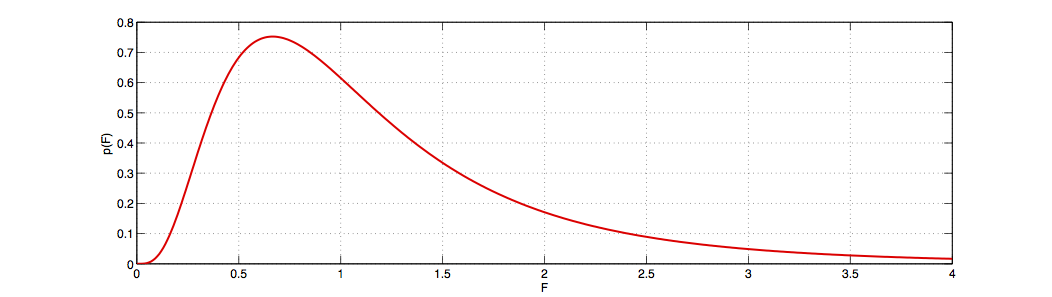
\includegraphics[width=0.8\textwidth]{fish.png}
    \end{center}
    }

    \only<2>{
    Предположения метода:
    \begin{enumerate}
    \item распределения признака во всех группах нормально;
    \item дисперсия значений признака во всех группах одинакова;
    \item наблюдения независимы.
    \end{enumerate}

    \bigskip

	\begin{itemize}
	\item Первое предположение считается выполненным, если распределение признака во всех группах нормально, или если объёмы выборок примерно одинаковы и $N-K-1\geq 20.$
	\item Второе предположение считается выполненным, если отношение наибольшей выборочной дисперсии к наименьшей не превосходит 10.
	\item При $n_1=\dots=n_K$ метод устойчив к нарушению первых двух предположений.
	\item Если объёмы выборок различаются, нарушение предположения о~равенстве дисперсий может привести к росту вероятности ошибки первого рода.
	\item Выбросы могут оказывать существенное влияние на результат.
	\end{itemize}
    }

%    \only<3>{
%    \textbf{Пример 1} (Bonnini, табл. 3.1): измерен вес пятидесяти пятиграммовых пакетиков сахара, расфасованы пятью разными производителями. 
%    Зависит ли от производителя средний вес сахара в пакетиках?
%    
%    \begin{figure}
%    	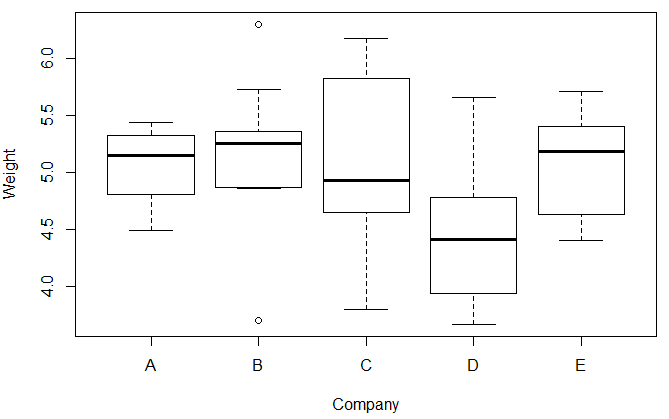
\includegraphics[width=0.7\textwidth]{sugar.png}
%    \end{figure}
%    
%    $H_0 \colon$ средний вес сахара одинаков для всех производителей.
%    
%    $H_1 \colon$ у каких-то производителей средний вес сахара отличается от~остальных. $\Rightarrow p = 0.115.$
%    }
    
    \only<3>{
    \begin{block}{Пример, Bonnini, табл. 3.2} Исследуется эффективность четырёх жаропонижающих средств, в составе которых один и тот же активный ингредиент присутствует в разных дозировках. Для каждой из четырёх групп из 15~морских свинок известно изменение температуры после введения жаропонижающего. Есть ли различия в действии препаратов?
    \end{block}
    \begin{figure}
    	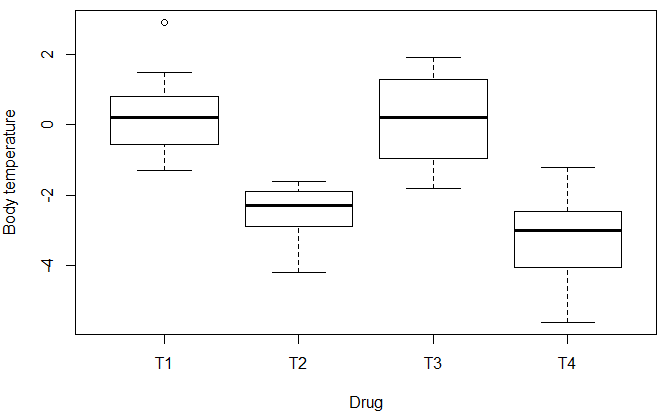
\includegraphics[width=0.45\textwidth]{drugs.png}
    \end{figure}    
    
    $H_0 \colon$ температура меняется в среднем одинаково.
    
    $H_1 \colon$ для каких-то препаратов среднее изменение температуры отличается от остальных.
    }
    
    \only<4>{
    \begin{figure}
    	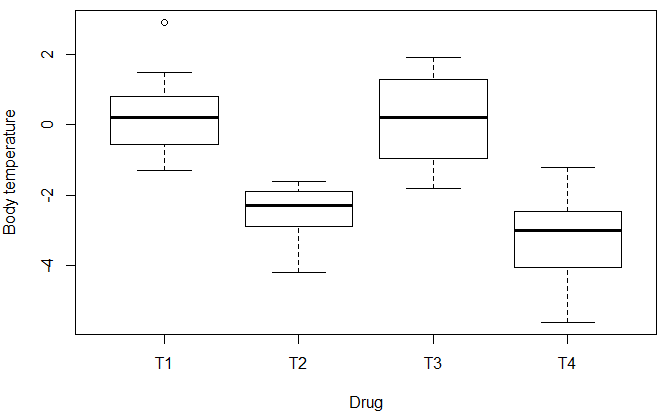
\includegraphics[width=0.55\textwidth]{drugs.png}
    \end{figure} 
    
    Критерий Фишера:
    \begin{center}
    	\begin{tabular}{cccccc}
    		          &  Df & Sum Sq & Mean Sq & F value &  Pr(>F)  \\
    		drug      &   3 & 143.0  & 47.67   & 40.21   & 5.43e-14 \\
    		Residuals &  56 &  66.4  &  1.19   &         &  \\              
    	\end{tabular}
    \end{center}        	
    }
\end{frame}

\begin{frame}[label=mannwhitney]{Критерий Манна-Уитни-Уилкоксона}
%%%%%%%%%%%%%%%%%%%%%%%%%%%%%%%%%%%%%%%%%%%%%%%%%%%%%%%%%%%%%%%%%%%%%%%
% Относительно параметра ? альтернатива в этом критерии может быть одностороннеи? или двустороннеи?. Если справедлива альтернативная гипотеза и между распределениями деи?ствительно есть сдвиг, то средние значения признаков в выборках будут различаться. Поэтому это тоже в каком-то виде гипотеза о средних.
%%%%%%%%%%%%%%%%%%%%%%%%%%%%%%%%%%%%%%%%%%%%%%%%%%%%%%%%%%%%%%%%%%%%%%%
   \begin{center}
     \begin{tabular}{rl}
         выборки:                        & $X_1^{n_1}=\left(X_{11},\ldots,X_{1n_1}\right)$         \\
                                         & $X_2^{n_2} = \left(X_{21},\ldots,X_{2n_2}\right)$ \\ 
                                         & выборки независимые\\
         нулевая гипотеза:               & $H_0\colon F_{X_1}\left(x\right) = F_{X_2}\left(x\right)$ \\
         альтернатива:                   & $H_1\colon F_{X_1}\left(x\right) = F_{X_2}\left(x+\Delta\right), \Delta <\neq> 0$ \\
         статистика:                     & $X_{(1)}\leq\ldots\leq X_{(n_1+n_2)}$ --- вариационный ряд \\
                                         & объединённой выборки $X = X_1^{n_1} \bigcup X_2^{n_2}$ \\
                                         & $R_1\left(X_1^{n_1}, X_2^{n_2}\right) = \sum\limits_{i=1}^{n_1} \rank\left(X_{1i}\right)$ \\
         нулевое распределение:          & табличное\\
     \end{tabular}
     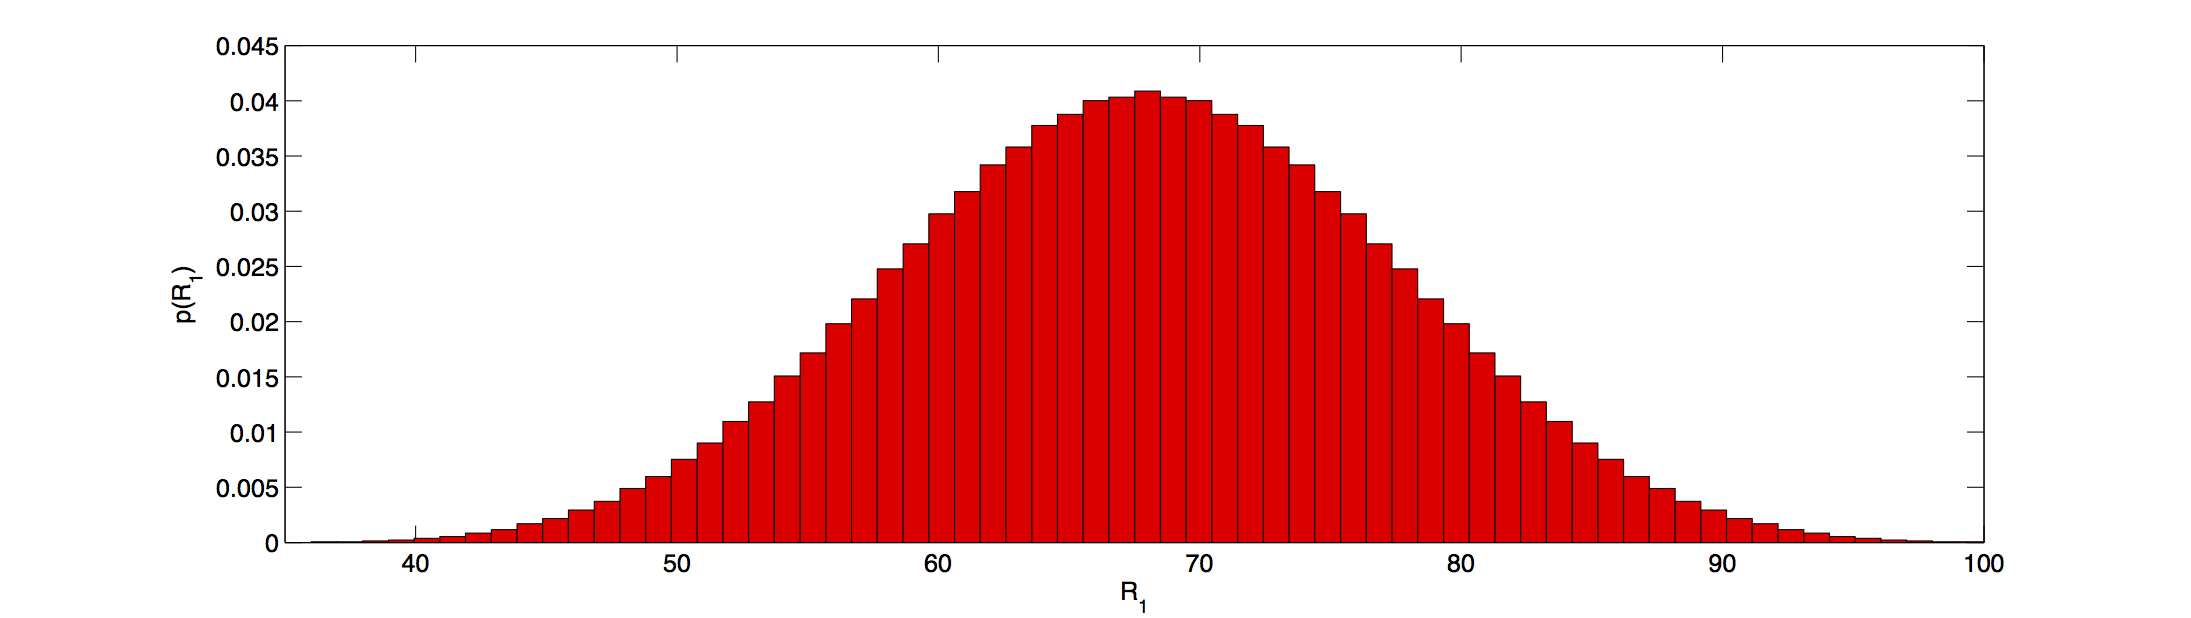
\includegraphics[width=0.8\textwidth]{mann.png}
 \end{center}
 
\end{frame}

\begin{frame}{Критерий Краскела-Уоллиса}
    \vspace{-10pt}
    
    \begin{center}
        \begin{tabular}{rl}
            выборки:                        & $X^N = X_1^{n_1}\bigcup\ldots\bigcup X_K^{n_K}, \;\; X_{k} \sim F\left(x + \Delta_k\right)$ \\
            нулевая гипотеза:               & $H_0\colon \Delta_1 = \Delta_2 = \ldots = \Delta_K$ \\
            альтернатива:                   & $H_1\colon H_0$ неверна\\
            статистика:                     & $K\left(X^N\right) = \left(N-1\right)\frac{\sum\limits_{k=1}^K n_k \left(\bar{r}_k-\bar{r}\right)^2 }{\sum\limits_{k=1}^K \sum\limits_{i=1}^{n_k} \left(r_{ki} - \bar{r}\right)^2}, \; r_{ki} \equiv \rank \left(X_{ki}\right)$\\
            нулевое распределение:          & табличное\\
        \end{tabular}
    \end{center}
    Если нет связок, то:
    $$\bar{r} = \frac{N-1}{2}, \sum\limits_{k=1}^K \sum\limits_{i=1}^{n_k} \left(r_{ki} - \bar{r}\right)^2 = \frac{\left(N-1\right) N \left( N+1\right) }{12}, $$
     $$   K\left(X^N\right) = \frac{12}{N\left(N+1\right)} \sum\limits_{k=1}^K n_k \bar{r}_k^2 - 3\left(N+1\right). $$

    Аппроксимация для $n_k>5$:
    $$K\left(X^N\right) \sim \chi^2_{K-1}.$$
	
	\bigskip	

    В предыдущем примере: $p=1.5\times 10^{-9}.$
\end{frame}


\begin{frame}{Критерий Джонкхиера}
    \only<1>{

    \begin{block}{Пример 1}
    Имеется гипотеза о том, что по мере перехода на старшие курсы падает посещаемость лекций. Для выяснения, верно ли это предположение, декан организовал выборочный контроль студентов. Случайным образом было отобрано некоторое одинаковое для каждого курса количество человек, а также был организован учет посещенных им лекций, отобранных случайно на каждом курсе. Требуется по данным учета проверить гипотезу.
    \end{block}
 
    \begin{block}{Пример 2}
    Взяты несколько групп пациентов, и каждой из них назначается определенная доза препарата.  Нужно проверить, как лекарство помогает в снятии соответствующего симптома.
    \end{block}
    }

    \only<2>{
    \begin{center}
        \begin{tabular}{rl}
            выборки:                        & $X^N = X_1^{n_1}\bigcup\ldots\bigcup X_K^{n_K}, \;\; X_{k} \sim F\left(x + \Delta_k\right)$ \\
            нулевая гипотеза:               & $H_0\colon \Delta_1 = \Delta_2 = \ldots = \Delta_K $ \\
                                            & \; $\Rightarrow \; \med X_1 = \ldots = \med X_K$ \\
            альтернатива:                   & $H_1\colon \med X_1 \leq \ldots \leq \med X_K$\\
            статистика:                     & $S\left(X^N\right) = \sum\limits_{k=1}^K \sum\limits_{i=1}^{n_k} a_{ki}$\\
                                            & $a_{ki}$~--- число наблюдений из первых $k-1$~выборок \\
                                            & меньших, чем $X_{ki}$ \\
            нулевое распределение:          & табличное\\
        \end{tabular}
    \end{center}

    \bigskip

    Аппроксимация для $n_k>10$:
    \begin{align*}
        S\left(X^N \right) &\sim N\left(\mu,\sigma^2\right),\\
        \mu &= \frac1{4}\left(N^2 - \sum\limits_{k=1}^{K} n_k^2\right),\\
        \sigma &=\frac1{72} \left( N^2\left(2N+3\right) -\sum\limits_{k=1}^K n_k^2\left(2n_k+3\right) \right).
    \end{align*}
    }

    \only<3>{
    \begin{block}{Пример,Bonnini, табл. 3.4} Исследуется зависимость предела прочности (в Ньютонах на квадратный метр) армированного бетона с разной концентрацией присадки~--- 16, 20, 24 и 28\%. Меняется ли средний предел прочности вместе с уровнем присадки?
    \end{block}
    \begin{figure}
    	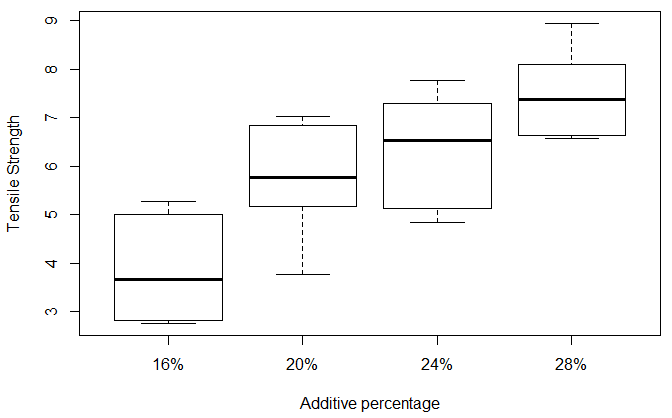
\includegraphics[width=0.45\textwidth]{concrete.png}
    \end{figure}        
%    исследуется влияние информированности (знания цели работы) на выполнение монотонных производственных операций. 18 рабочих были случайным образом разделены на 3 группы. Попавшие в группу 1 не~имели информации о требуемой производительности, в группу 2~--- получили общее представление о том, что нужно делать, в группу 3~--- точную информацию о задании и график выполнения работ.

    $H_0 \colon$ концентрация присадки не влияет на среднюю прочность.

    $H_1 \colon$ концентрация присадки влияет на среднюю прочность $\Rightarrow p = 0.0042.$

    $H_1 \colon$ увеличение концентрации присадки повышает среднюю прочность $\Rightarrow p = 2.936\times 10^{-5}.$
    }
\end{frame}

\subsection{Вторичный анализ}
\begin{frame}{Модель со случайным эффектом}
    \only<1>{
    \begin{itemize}
    \item Характеристика, определяющая разбиение на группы, не~представляет непосредственного интереса.
    \item Группы случайно выбраны из множества возможных групп.
    \item Если между группами есть неоднородность, ожидается, что она сохранится при повторе эксперимента, но соотношения между средними могут измениться.
    \end{itemize}

    \bigskip

    Примеры.
    \begin{itemize}
    \item Размеры горбаток в разных семьях, выращенных на одном и том же растении; цель --- определить значимость фактора семьи для дальнейших исследований.
    \item Уровень гликогена в различных образцах икроножной мышцы крысы; если вариация между образцами даёт маленький вклад в общую вариацию,  то можно считать, что для измерения уровня достаточно одного образца.
    \item Вкусовые качества персиков с 10 различных деревьев; планируется сравнить различия во вкусовых качествах персиков с разных деревьев с различиями у персиков с одного дерева. Если последние больше, то~бессмысленно выбрать для размножения дерево с лучшей средней оценкой.
    \end{itemize}
    }

    \only<2>{
    Если используется \textbf{модель со случайным эффектом}, следующий шаг~--- разделение дисперсий на внутригрупповые и межгруповые.

    \bigskip

	Доля межгрупповой дисперсии в общей дисперсии выборки:
	$$\eta^2 = \frac{SS_{bg}}{SS_{total}};$$

	в популяции:
	
	$$\hat{\omega}^2 = \frac{SS_{bg} - SS_{wg} \left(K-1\right)/ \left(N-K\right)}{SS_{total} + SS_{wg}/\left(N-K\right)}.$$
    }
\end{frame}

\begin{frame}{Модель с фиксированным эффектом}
    \only<1>{
    \begin{itemize}
    \item Разбиение на группы определено до получения данных.
    \item При повторе эксперимента ожидается, что соотношения между средними групп сохранятся.
    \item Если между средними есть различия, на следующем этапе анализируется, какие именно группы различаются.
    \end{itemize}

    \bigskip

    Примеры.
    \begin{itemize}
    \item Продолжительность жизни разноногих раков в морской воде и~растворах глюкозы и маннозы.
    \item Экспрессия определённого гена в тканях мозга, печени, лёгких и~мышц; необходимо понять, в какой ткани экспрессия выше.
    \item Вкусовые качества персиков с 10 различных деревьев; планируется выбрать лучшее дерево для дальнейшего разведения.
    \end{itemize}
    }

    \only<2>{
    Если используется \textbf{модель с фиксированным эффектом}, то, в случае отвержения гипотезы однородности средних, проводится дополнительное сравнение с целью уточнения характера различий.

    Сравнение может быть:
    \begin{itemize}
    \item запланированным, когда группы для дальнейшего сравнения отобраны до сбора данных.
    \item незапланированным (post hoc), когда группы для сравнения выбираются по~результатам первичного анализа данных.
    \end{itemize}

    Для запланированного попарного сравнения групп можно просто использовать подходящий двухвыборочный критерий.

    Для незапланированного сравнения всё сложнее.
    }
\end{frame}

\begin{frame}{Критерий Даннета}
    \begin{align*}
    D_i &= \frac{\bar{X}_i-\bar{X}_1}{S\sqrt{\frac1{n_i} + \frac1{n_1}}}, \\
    S^2 &= \frac1{N-K} \sum\limits_{k=1}^K \left(n_k-1\right)S_k^2, \\
    \intertext{где $S_k^2$ --- дисперсия выборки $X_k^{n_k}$.}
    \end{align*}
    
    \vspace{-20pt}
    
    Если $X_{i,j}\sim N\left(\mu_i, \sigma^2\right),$ то при $\mu_1=\dots=\mu_K$ вектор $D = \left(D_2,\dots,D_k\right)$ имеет многомерное распределение Стьюдента.

    Кроме того, для $D$  можно построить процедуру, контролирующую FWER. 
    
    \bigskip
    
\end{frame}

\begin{frame}{LSD Фишера (Least Significant Difference)}
    Если $\alpha_i=\alpha_j,$ то
    $$\frac{\bar{X}_i - \bar{X}_j}{S \sqrt{\frac1{n_i} + \frac1{n_j}}} \sim St\left(n_i + n_j - 2\right),$$
    где $S^2 = \frac{\left(n_i-1\right)S_i^2 + \left(n_j-1\right)S_j^2}{n_i + n_j - 2}.$

    Рассмотрим величину
    $$LSD_{ij} = \frac{t_{\alpha} S}{\sqrt{\frac1{n_i} + \frac1{n_j}}},$$
    где $t_{\alpha}$~--- $\alpha$-квантиль распределения Стьюдента с $n_i + n_j - 2$ степенями свободы.

    \bigskip

    Если $\left|\bar{X}_i - \bar{X}_j\right|>LSD_{ij},$ то частная нулевая гипотеза $H_0\colon \alpha_i = \alpha_j$ отклоняется против двусторонней альтернативы.

    \bigskip

    LSD можно использовать только в случае отвержения общей гипотезы однородности.
    
    \textbf{Не контролирует FWER/FDR.}
\end{frame}

\begin{frame}
    \frametitle{HSD Тьюки (Honest Significant Difference)}
    \begin{align*}
        n   &= \frac{K}{\sum\limits_{k=1}^K \frac1{n_k}}, \\
        S^2 &= \frac1{N-K} \sum\limits_{k=1}^K \left(n_k-1\right)S_k^2, \\
        \intertext{где $S_k^2$ --- дисперсия выборки $X_k^{n_k}$,}
        HSD &= \frac{q_{\alpha}\left(N-K\right)S}{\sqrt{n},}
    \end{align*}
    где $q_{\alpha}\left(N-K\right)$~--- критическое значение распределения стьюдентизированного размаха с $N-K$ степенями свободы.

    \bigskip

    Если $\left|\bar{X}_i - \bar{X}_j\right|>HSD,$ то частная нулевая гипотеза $H_0\colon \alpha_i = \alpha_j$ отклоняется против двусторонней альтернативы.

    \bigskip

    HSD можно использовать независимо от справедливости общей гипотезы однородности.\\
   \textbf{Контролирует FWER.}
\end{frame}

\begin{frame}{Критерий Неменьи}
    Ранговый аналог HSD.
    $$    CD = q'_{\alpha} \sqrt{\frac{K\left(K+1\right)}{6N}},$$
    где $q'_{\alpha}$~--- критическое значение статистики критерия, основанное на распределении стьюдентизированного размаха.

    \bigskip

    Если $\left|\bar{r}_i - \bar{r}_j\right|>CD,$ то частная нулевая гипотеза $H_0\colon \Delta_i = \Delta_j$ отклоняется против двусторонней альтернативы.
\end{frame}


\begin{frame}{Post-hoc критерии: резюме}
\begin{itemize}
\item Распределение в группах нормально, требуется сравнить одну группу с остальными: критерий Данннета.
\item Распределение в группах нормально, требуется сравнить все группы со всеми: HSD Тьюки.
\item Распределение в группах не нормально, требуется сравнить все группы со всеми: критерий Немени.
\end{itemize}
\end{frame}

\begin{frame}{Пример} 
	\only<1>{
    Действие жаропонижающих на морских свинок:
    
    \begin{figure}
    	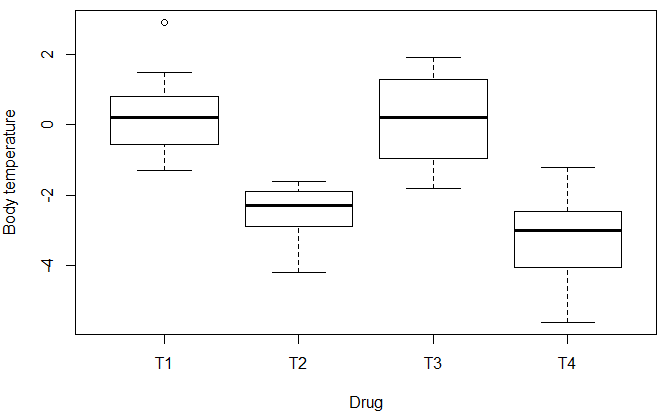
\includegraphics[width=0.4\textwidth]{drugs.png}
    \end{figure}    
        
    HSD:
        \begin{center}
        	\begin{tabular}{crrrr}           
                                &  diff        &      lwr   &       upr   &    p adj \\
                         T2-T1  & $-2.72666667$  & $-3.779467$  & $-1.6738668$  & $0.0000000$\\
                         T3-T1  & $-0.06666667$  & $-1.119467$  & $ 0.9861332$  & $0.9983032$\\
                         T4-T1  & $-3.43333333$  & $-4.486133$  & $-2.3805335$  & $0.0000000$\\
                         T3-T2  & $ 2.66000000$  & $ 1.607200$  & $ 3.7127999$  & $0.0000001$\\
                         T4-T2  & $-0.70666667$  & $-1.759467$  & $ 0.3461332$  & $0.2949015$\\
                         T4-T3  & $-3.36666667$  & $-4.419467$  & $-2.3138668$  & $0.0000000$    \\    
        	\end{tabular}
        \end{center}    

    
%    \begin{center}\small
%    \begin{tabular}{|c|c|c|c|} \hline
%       & T1                   &  T2                & T3 \\ \hline
%	T2 & $3.5\times10^{-8}$   & -                  & - \\
%	T3 & $0.9983$             & $6.7\times10^{-8}$ & - \\
%	T4 & $4.95\times10^{-11}$ & $0.2949$           & $8.6\times10^{-11}$ \\ \hline
%    \end{tabular}
%    \end{center}    

	}
	\only<2>{
    Действие жаропонижающих на морских свинок:
    
    \begin{figure}
    	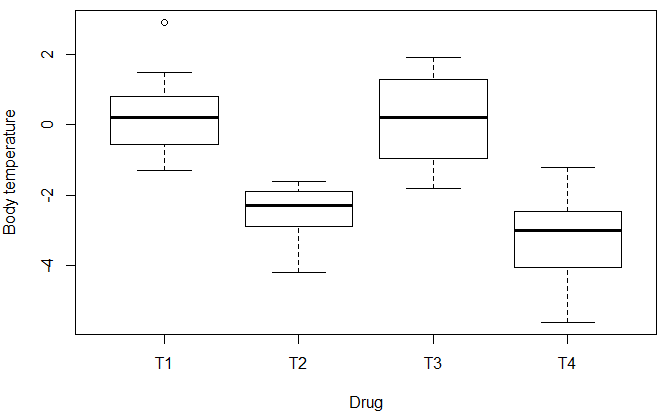
\includegraphics[width=0.4\textwidth]{drugs.png}
    \end{figure}  
        
    \bigskip
    
    Критерий Неменьи:
    \begin{center}\small
    	\begin{tabular}{cccc}
    		& T1                 & T2        & T3 \\ 
    		T2 & $0.00016$          & -         & - \\
    		T3 & $0.99999$          & $0.00018$ & - \\
    		T4 & $1.9\times10^{-6}$ & $0.79418$ & $2.2\times10^{-6}$ \\ 
    	\end{tabular}
    \end{center}    
	}
\end{frame}

\subsection{Сравнение дисперсий}
\begin{frame}{Критерий Бартлетта}
    \only<1>{
%    \vspace{-15pt}
    \begin{center}
        \begin{tabular}{rl}
            выборки:                        & $X^N = X_1^{n_1}\bigcup\ldots\bigcup X_K^{n_K}, \;\; X_{ki} \sim N\left(\mu_k, \sigma^2_k\right)$ \\
            нулевая гипотеза:               & $H_0\colon \sigma_1 = \sigma_2 = \ldots = \sigma_K$ \\
            альтернатива:                   & $H_1\colon H_0$ неверна\\
            статистика:                     & $B\left(X^N\right) = \frac{\ln 10}{C} \left(\left(N-K\right)\ln S^2 - \sum\limits_{k=1}^K \left(n_k-1\right)\ln S_k^2\right)$ \\
                                            & $S^2 = \frac1{N-K} \sum\limits_{k=1}^K \left(n_k-1\right) S_k^2$\\
                                            & $C = 1 + \frac1{3K+1}\left(\sum\limits_{k=1}^K \frac1{n_k-1} - \frac1{N}\right)$\\
            нулевое распределение:          & табличное\\
        \end{tabular}
    \end{center}
    Аппроксимация для $n_k>6$:
    $$B\left(X^N\right)\sim\chi^2_{K-1}.$$
    }

    \only<2>{
    \begin{block}{Пример, Beall, 1942} Шесть видов инсектицидов тестируется на 12 полях каждый, исследуемый признак~--- количество насекомых на поле через некоторое время после обработки.
    \end{block}

    \begin{figure}
    	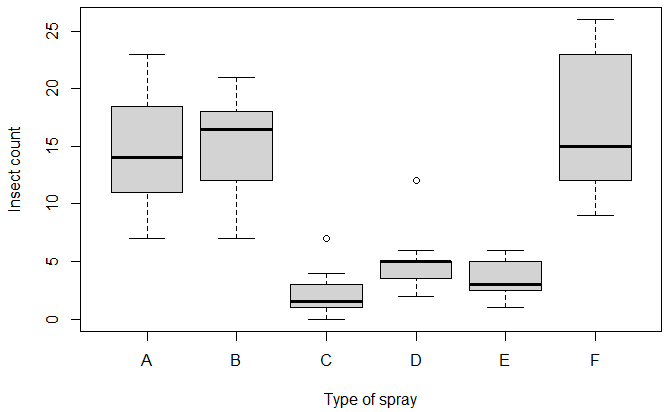
\includegraphics[width=0.4\textwidth]{insectspray.png}
    \end{figure}

    \bigskip

    $H_0 \colon$ дисперсия числа насекомых на полях, обрабатываемых разными инсектицидами, одинакова.

    $H_1 \colon$ дисперсия числа насекомых на полях, обрабатываемых разными инсектицидами, неодинакова $\Rightarrow p = 9\times10^{-5}.$
    }
\end{frame}


\section{2-way b.s.}
\subsection{Омнибус-критерии}
\begin{frame}{Двухфакторный дисперсионный анализ}
    \only<1>{
    $f_1\colon X \rightarrow \left\{1,\ldots,K_1\right\}, \;\; f_2 \colon X \rightarrow \left\{1,\ldots,K_2\right\}$

    \bigskip

    \begin{center}
    \begin{tabular}{|c|c|c|c|c|c|}
    \hline
    \diagbox{$f_1$}{$f_2$} & $1$ & $\ldots$ & $j$ & $\ldots$ & $K_2$ \\\hline
    $1$        &&&&& \\\hline
    $\vdots$ &&&&& \\\hline
    $i$      &&&  $\footnotesize{\begin{matrix} X_{ij1} \\ \vdots \\ X_{ijn_{ij}} \end{matrix}}$ && \\\hline
    $\vdots$ &&&&& \\\hline
    $K_1$    &&&&& \\\hline
    \end{tabular}
    \end{center}

    \bigskip

    Задача: проверить гипотезу об отсутствии влияния факторов $f_1$ и $f_2$ на~среднее значение признака $X$.
    
    Случай выборок разного размера для двух факторов значительно сложнее, поэтому будем считать, что $n_{11} = \ldots = n_{K_1 K_2} = n$.
    }

    \only<2>{
    Линейная модель:
    $$X_{ijk} = \mu + \alpha_i + \beta_j + \gamma_{ij} + \varepsilon_{ijk}, $$

    $i=1,\ldots,K_1, \; j=1,\ldots,K_2, \; k=1,\ldots,n.$

    \bigskip

    $\mu$~--- общее среднее значение признака,

    $\alpha_i$~--- воздействие уровня $i$ фактора $f_1$,

    $\beta_j$~---  воздействие уровня $j$ фактора $f_2$,

    $\gamma_{ij}$~--- дополнительное воздействие комбинации уровней $i$ и $j$ факторов $f_1$~и~$f_2$,

    $\varepsilon_{ijk}$~--- случайные независимые одинаково распределённые ошибки.
    }

    \only<3>{
    \begin{align*}
    H_0^1\colon & \text{фактор $f_1$ не влияет на значение признака } X \Leftrightarrow \\
                & \alpha_i=0 \;\; \forall i,\\
    H_1^1\colon & f_1 \text{ влияет на значение } X;\\
    \end{align*}

    \begin{align*}
    H_0^2\colon & \text{фактор $f_2$ не влияет на значение признака } X \Leftrightarrow \\
                & \beta_j=0 \;\; \forall j, \\
    H_1^2\colon & f_2 \text{ влияет на значение } X;\\
    \end{align*}

    \begin{align*}
    H_0^{12}\colon & \text{между факторами $f_1, f_2$ нет взаимодействия} \Leftrightarrow \\
                   & \gamma_{ij}=0 \;\; \forall i,j,\\
    H_1^{12}\colon & \text{ между факторами $f_1, f_2$ есть взаимодействие.}\\
    \end{align*}
    }

    \only<4>{
    \textbf{Пример:} $X$~--- успешность решения задачи (в баллах от 0 до 10),

    $f_1$~--- размер команды (1~--- маленькая, 2~--- средняя, 3~--- большая),

    $f_2$~--- наличие назначенного лидера (1~--- нет, 2~--- есть).

    \bigskip

    \begin{center}
        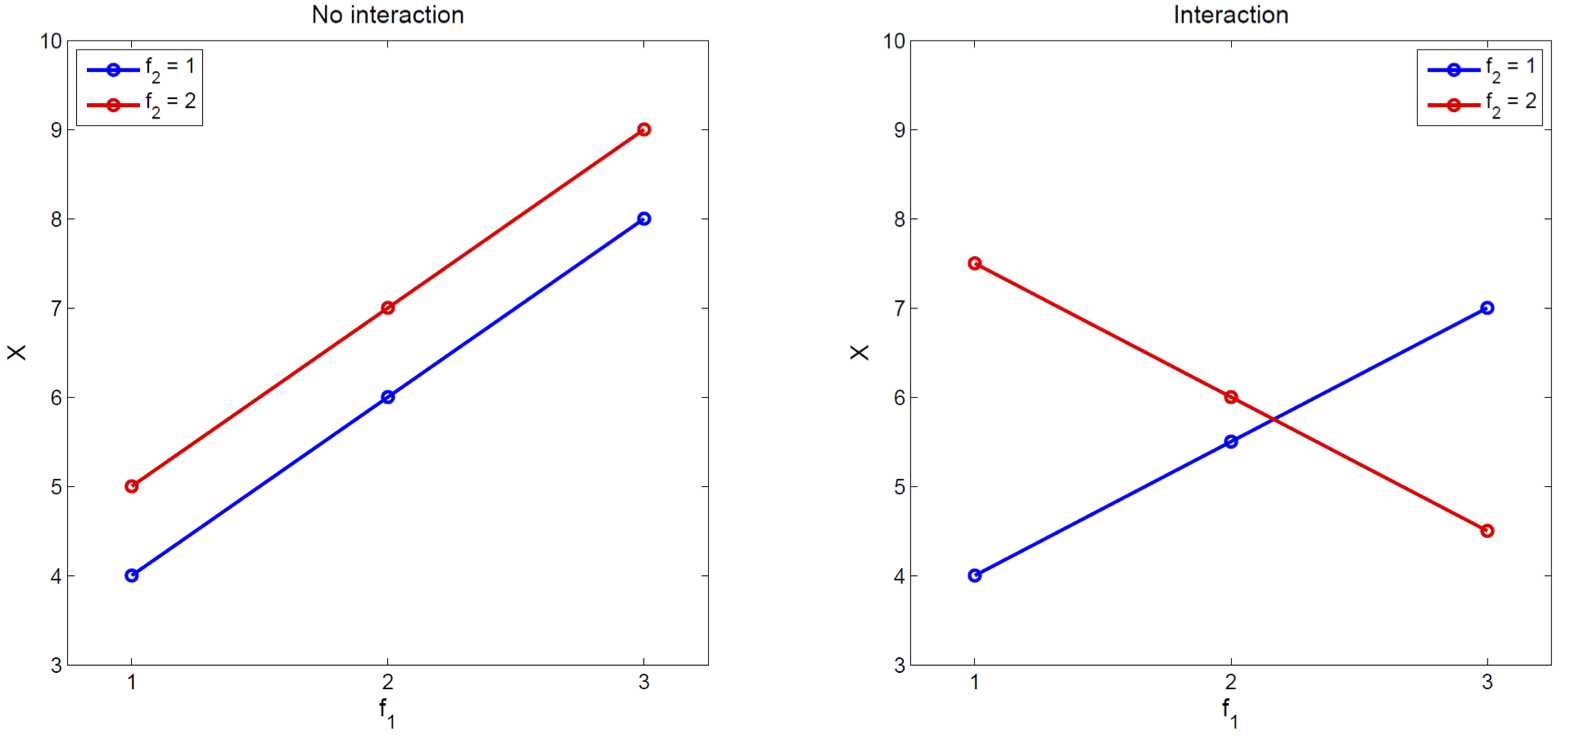
\includegraphics[width=0.7\textwidth]{interactions.png}
    \end{center}
    }
\end{frame}

\subsection{Параметрический вариант}
\begin{frame}{Нормальный двухфакторный дисперсионный анализ}
    \only<1>{
    %НЕТ
    
    Предположим, что $X_{ijk} \sim N\left(\mu_{ij}, \sigma^2\right)$ $\Leftrightarrow \varepsilon_{ijk} \sim N\left(0,\sigma^2\right)$.

    $\bar{X}_{ij}$~--- среднее в ячейке,

    $\bar{X}_{i \bullet}$~--- среднее по строке $i$,

    $\bar{X}_{\bullet j}$~--- среднее по столбцу $j$,

    $\bar{X}$~--- среднее по всей таблице.

    Внутрифакторные дисперсии:

    \begin{align*}
        S_1^2    &= \frac{nK_2}{K_1-1} \sum\limits_{i=1}^{K_1} \left(\bar{X}_{i \bullet} - \bar{X}\right)^2, \\
        S_2^2    &= \frac{nK_1}{K_2-1} \sum\limits_{i=1}^{K_2} \left(\bar{X}_{\bullet j} - \bar{X}\right)^2, \\
        S_{12}^2 &= \frac{n}{\left(K_1-1\right)\left(K_2-1\right)} \sum\limits_{i,j} \left(\bar{X}_{ij} - \bar{X}_{i \bullet} - \bar{X}_{\bullet j} + \bar{X}\right)^2, \\
        S_{res}^2&= \frac1{K_1 K_2\left(n-1\right)} \sum\limits_{k=1}^{n} \sum\limits_{i,j} \left(X_{ijk} - \bar{X}_{i j}\right)^2. \\
    \end{align*}
    }

    \only<2>{
    Проверка значимости факторов и их взаимодействия:
    \begin{itemize}
    \item $n>1$:
    \begin{align*}
        F_1    &= \frac{S_1^2}{S_{res}^2} \sim F\left(K_1-1, K_1K_2\left(n-1\right)\right) \text{ при } H_0^1, \\
        F_2    &= \frac{S_2^2}{S_{res}^2} \sim F\left(K_2-1, K_1K_2\left(n-1\right)\right) \text{ при } H_0^2, \\
        F_{12} &= \frac{S_{12}^2}{S_{res}^2} \sim F\left(\left(K_1-1\right)\left(K_2-1\right), K_1K_2\left(n-1\right)\right) \text{ при } H_0^{12}; \\
    \end{align*}
    \item $n=1$:
    \begin{align*}
        F_1    &= \frac{S_1^2}{S_{12}^2} \sim F\left(K_1-1, \left(K_1-1\right)\left(K_2-1\right) \right) \text{ при } H_0^1, \\
        F_2    &= \frac{S_2^2}{S_{12}^2} \sim F\left(K_2-1, \left(K_1-1\right)\left(K_2-1\right) \right) \text{ при } H_0^2. \\
    \end{align*}
    При этом подразумевается, что $H_0^{12}$ верна.
    \end{itemize}
    }
\end{frame}

\begin{frame}{Марихуана и скорость реакции}
    \only<1>{
    \begin{block}{Пример, Pagano, 2012, задача 16.2} Изучалось воздействие марихуаны на скорость реакции. В~качестве испытуемых были выбраны по 12 человек из каждой категории:
    \begin{itemize}
    \item никогда не пробовали марихуану;
    \item иногда употребляют марихуану;
    \item регулярно употребляют марихуану.
    \end{itemize}
    Испытуемые были разделены на две равные группы; половине из них дали выкурить две сигареты с марихуаной, вторая половина выкурила две обычные сигареты с запахом и вкусом марихуаны. Сразу после этого все испытуемые прошли тест на скорость реакции.

    Требуется оценить влияние марихуаны на скорость реакции, учитывая фактор предыдущего опыта употребления.
    \end{block}
    }

    \only<2>{
    \begin{center}    	
		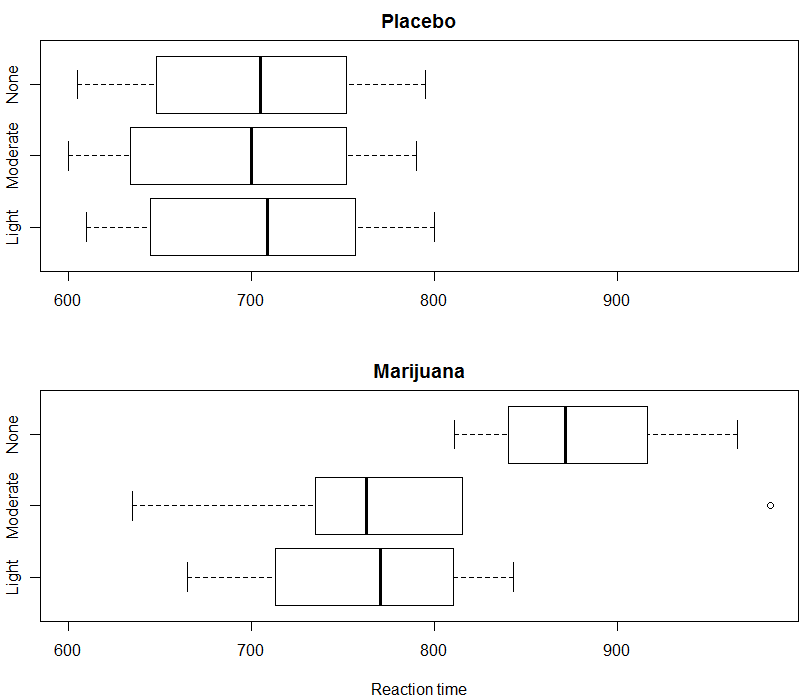
\includegraphics[height=0.7\textheight]{weed.png}
	\end{center}
    }

    \only<3>{
    $H_0^1\colon$ средняя скорость реакции одинакова при употреблении и~марихуаны, и~сигарет.

    $H_0^2\colon$ средняя скорость реакции не зависит от предыдущего опыта употребления марихуаны.

    $H_0^{12}\colon$ отсутствует межфакторное взаимодействие между употребляемым веществом и предыдущим опытом употребления марихуаны.

    \bigskip

    \begin{center}
     \begin{tabular}{lccccc}
                                        & Df   &Sum Sq   &Mean Sq   &F value   &  Pr(>F)    \\
                                        Treatment           &  $1$ &$103041$ & $103041$ & $17.584$ &$0.000224$\\
                                        Past usage          &  $2$ &$ 23634$ & $ 11817$ & $ 2.017$ &$0.150752$            \\            
                                        Past usage:Treatment&  $2$ &$ 23642$ & $ 11821$ & $ 2.017$ &$0.150665$    \\
                                        Residuals           & $30$ &$175796$ & $  5860$ &          &                  
     \end{tabular}
     \end{center}
     

    }

    \only<4>{
    Вывод: гипотеза о том, что предыдущий опыт употребления не влияет на скорость реакции, не отклоняется $\Rightarrow$ данные по группам можно объединить.

	\bigskip

	\begin{center}    	
		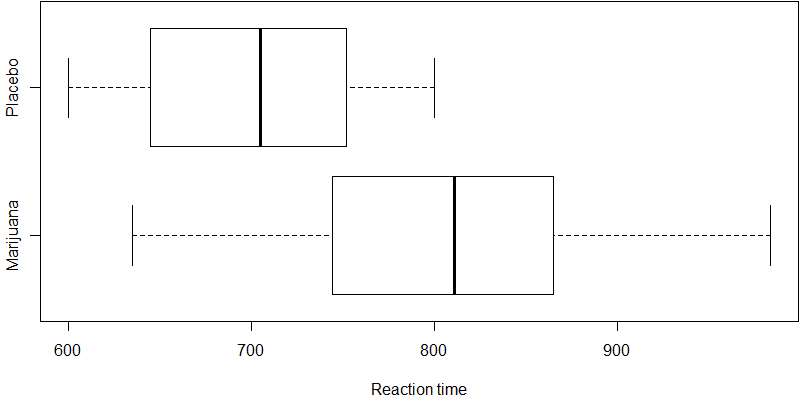
\includegraphics[width=0.65\textwidth]{weed2.png}
	\end{center}     

	\bigskip

    Для объединённых данных:
    \begin{itemize}
    \item однофакторный дисперсионный анализ: $p=0.0004;$
    \item критерий Стьюдента, односторонняя альтернатива: $p=0.0002$, 95\%~нижний доверительный предел~--- $61.2$.
    \end{itemize}
    }
    
%    \only<5>{
%    \textbf{Пример 2}: витамин C и рост зубов
%    	
%	\url{https://yadi.sk/d/mPb2G8cqf52as}    
%    }
\end{frame}

\subsection{Иерархический дизайн}
\begin{frame}{Иерархический дизайн}
    Стандартная постановка двухфакторного дисперсионного анализа предполагает, что уровни факторов в выборке распределены независимо.

    \bigskip

    Пример, когда это не так: 
    
    признак --- уровень гликогена в икроножной мышце крысы, 
    
    фактор~1~--- уровень стресса крыс,
    
    фактор~2~--- различия между клетками. 
    
    Крысы со стрессом живут в клетках~1~и~2, без стресса --- 3~и~4.

    \bigskip

    Решение --- иерархический дисперсионный анализ.
    
    \textbf{Линейная модель:}
    $$X_{ijk} = \mu + \alpha_i + \beta_{ij} + \varepsilon_{ijk}, $$
    фактор $j$ теперь зависит от фактора $i$.

\end{frame}

\begin{frame}
    \frametitle{CBI чернобрюхой дрозофилы}
    \only<1>{
    Codon bias index (CBI) --- мера случайности использования синонимичных кодонов в геноме --- была определена для нескольких регионов двух хромосом чернобрюхой дрозофилы.
    Требуется определить, есть ли систематические различия по величине CBI между разными хромосомами и регионами.

    \bigskip

    \begin{center}
        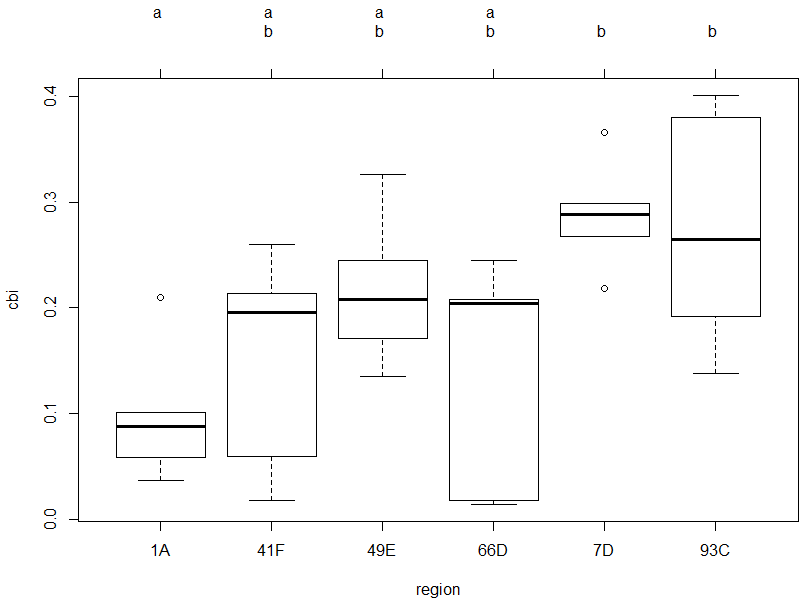
\includegraphics[height=0.45\textheight]{fly.png}
    \end{center}
    }

    \only<2>{
    \begin{center}
     \begin{tabular}{cccccc}
                          & Df   &  Sum Sq    & Mean Sq   & F value   &  Pr(>F)   \\
                          Chromosome        & $2$  & $0.01033$  & $0.00516$ &   $0.657$ & $0.52554$   \\
                          Chromosome:Region & $3$  & $0.16295$  & $0.05432$ &   $6.915$ & $0.00113$ \\
                          Residuals         & $30$ & $0.23564$  & $0.00785$ &           &  \\         
     \end{tabular}
     \end{center}
     
     \bigskip

     Есть различия между регионами, нет различий между хромосомами.
    }

    \only<3>{
     Для  уточнения различий применим метод HSD:
     
     \bigskip
     
    \begin{center}
     \begin{tabular}{llrrr}
     Группа 1 & Группа 2 & $CI_L$ & mean   & $CI_U$ \\
     7D       & 93C      & $-0.1485$& $0.0093$ & $0.1672$\\
     7D       & 49E      & $-0.0847$& $0.0732$ & $0.2310$\\
     7D       & 41F      & $-0.0161$& $0.1417$ & $0.2996$\\
     7D       & 1A       & $ 0.0181$& $0.1886$ & $0.3591$\\ %!
     7D       & 66D      & $-0.0207$& $0.1498$ & $0.3203$\\
     93C      & 49E      & $-0.0802$& $0.0639$ & $0.2079$\\
     93C      & 41F      & $-0.0117$& $0.1324$ & $0.2765$\\
     93C      & 1A       & $ 0.0214$& $0.1793$ & $0.3371$\\ %!
     93C      & 66D      & $-0.0174$& $0.1405$ & $0.2983$\\
     49E      & 41F      & $-0.0755$& $0.0686$ & $0.2127$\\
     49E      & 1A       & $-0.0424$& $0.1154$ & $0.2733$\\
     49E      & 66D      & $-0.0812$& $0.0766$ & $0.2345$\\
     41F      & 1A       & $-0.1110$& $0.0469$ & $0.2047$\\
     41F      & 66D      & $-0.1498$& $0.0081$ & $0.1659$\\
     1A       & 66D      & $-0.2093$&$-0.0388$ & $0.1317$\\
     \end{tabular}
     \end{center}
    }


\end{frame}

\subsection{Болтающийся контроль}
\begin{frame}
	\frametitle{Болтающаяся контрольная группа}

    \begin{center}
	\begin{tabular}{|c|c|c|c|}
		\cline{1-3}
		\diagbox{Лекарство}{Доза}  & 5 мг & 10 мг &  \multicolumn{1}{c}{} \\ \cline{1-3}
							Препарат А  &      &       &  \multicolumn{1}{c}{} \\ \cline{1-3}
							Препарат B  &      &       &  \multicolumn{1}{c}{} \\ \hline
						   \multicolumn{3}{c|}{}        &  Плацебо, 0 мг       \\ \cline{4-4}
	\end{tabular}
    \end{center}	
	
	\bigskip
	
	Используется однофакторный дисперсионный анализ с последующими запланированными сравнениями.	
\end{frame}

%\section{3-way b.s.}
%\subsection{Пример}
%\begin{frame}{Пример}
%	Лечение гипертонии:
%	
%	\url{https://yadi.sk/d/nHJk7_C4fGW38}
%	
%    \only<1>{
%    72 пациента проходили лечение от гипертонии. Для лечения использовались три вида лекарств, при этом их эффект изучался как при использовании специальной диеты, так и в её отсутствии; кроме того, в~ряде случаев применялась психотерапия. Данные~--- артериальное давление пациента по окончании лечения.
%
%    Требуется сравнить эффективность методов для лечения гипертонии.
%
%    \bigskip
%
%    Дизайн $[3\times2\times2].$
%    }
%
%    \only<2>{
%    Трёхфакторный дисперсионный анализ, все взаимодействия:
%
%    \bigskip
%
%    \begin{center}
%    \begin{tabular}{cccccc}
%    Source            & SS      & df  & MS       & F       & Prob>F  \\ \hline
%    Therapy           & $2048$  & $1$ & $2048$   & $13.07$ & $0.0006$\\
%    Diet              & $5202$  & $1$ & $5202$   & $33.2$  & $3\times10^{-7}$     \\
%    Drug              & $3675$  & $2$ & $1837.5$ & $11.73$ & $0.0001$\\
%    Therapy*Diet      & $32$    & $1$ & $32$     & $0.2$   & $0.6529$\\
%    Therapy*Drug      & $259$   & $2$ & $129.5$  & $0.83$  & $0.4425$\\
%    Diet*Drug         & $903$   & $2$ & $451.5$  & $2.88$  & $0.0638$\\
%    Therapy*Diet*Drug & $1075$  & $2$ & $537.5$  & $3.43$  & $0.0388$\\
%    Error             & $9400$  & $60$& $156.67$ &         &         \\
%    \end{tabular}
%    \end{center}
%
%	Воздействие одного из факторов различно при различных комбинациях двух других. 
%	Хотя эффект Therapy*Drug незначим в целом, значимость Therapy*Diet*Drug говорит о том, что влияние Therapy*Drug необходимо оценивать отдельно для пациентов, использующих и не использующих диету.
%    }
%                     
%    \only<3>{
%    	\begin{itemize}
%    		\item Для пациентов, соблюдающих диету:
%    \begin{center}
%    	\begin{tabular}{cccccc}
%    		Source            & SS      & df  & MS      & F       & Prob>F  \\ \hline
%    		Therapy           & $784$   & $1$ & $784.0$ & $4.436$ & $0.0437$\\
%    		Drug              & $474$   & $2$ & $237.0$ & $1.341$ & $0.2768$\\
%    		Therapy*Drug      & $182$   & $2$ & $91.0$  & $0.515$ & $0.6027$\\
%    		Error             & $5302$  & $30$& $176.7$ &         &         \\
%    	\end{tabular}
%    \end{center}    		
%    		
%    		 
%    		\item
%    	\end{itemize}
%    }
%\end{frame}

\section{1-way w.s.}
\subsection{Омнибус-критерии}
\begin{frame}{Однофакторный дисперсионный анализ для связанных выборок}
    \begin{center}
    \begin{tabular}{|c|c|c|c|c|c|}
    \hline
    \diagbox{Объект}{$f$} & $1$      & $\ldots$ & $k$      & $\ldots$ & $K$      \\ \hline
    1                           & $X_{11}$ &          & $X_{k1}$ &          & $X_{K1}$ \\ \hline
    $\vdots$                    & $\vdots$ & $\cdots$ & $\vdots$ & $\cdots$ & $\vdots$ \\ \hline
    $n$                         & $X_{1n}$ &          & $X_{kn}$ &          & $X_{Kn}$ \\ \hline
    \end{tabular}
    \end{center}

    \bigskip

    Линейная модель:
    $$X_{ki} = \mu + \alpha_k + \beta_i + \varepsilon_{ki},$$
    $i=1,\dots,n, \; k=1,\dots,K.$

    \bigskip

    $\mu$~--- глобальное среднее значение признака $X$,

	$\beta_i$~--- отклонение от $\mu$, вызванное влиянием особенностей $i$-го объекта,

    $\alpha_k$~--- отклонение от $\mu+\beta_i$, вызванное влиянием $k$-го уровня фактора $f$,

    $\varepsilon_{ki}$~--- случайные независимые одинаково распределённые ошибки.

    \bigskip

    Средние значения $X$ во всех $K$ выборках одинаковы $\Leftrightarrow$ $\alpha_1=\dots=\alpha_K$.
\end{frame}

\begin{frame}{Критерий Фишера}
    \only<1>{\small
    \begin{center}
        \begin{tabular}{rl}
            выборки:                        & $X^N = X_1^{n_1}\bigcup\ldots\bigcup X_K^{n_K}$ \\
            нулевая гипотеза:               & $H_0\colon \alpha_1 = \alpha_2 = \ldots = \alpha_K$ \\
            альтернатива:                   & $H_1\colon H_0$ неверна\\
            статистика:                     & $F\left(X^N\right) = \frac{SS_{bg}/ \left(K-1\right)}{\left(SS_{wg}-SS_{s}\right) / \left(n-1\right)\left(K-1\right)}$ \\
                                            & $SS_{bg} = n \sum\limits_{k=1}^K \left(\bar{X}_k - \bar{X}\right)^2$ \\
                                            & $SS_{wg} =   \sum\limits_{k=1}^K \sum\limits_{i=1}^{n} \left(X_{ki} - \bar{X}_k\right)^2$ \\
                                            & $SS_{s}  = K \sum\limits_{i=1}^n \left(\bar{X}_{i} - \bar{X}\right)^2$ \\
            нулевое распределение:          & $F(K-1, (n-1)(K-1))$\\
        \end{tabular}
        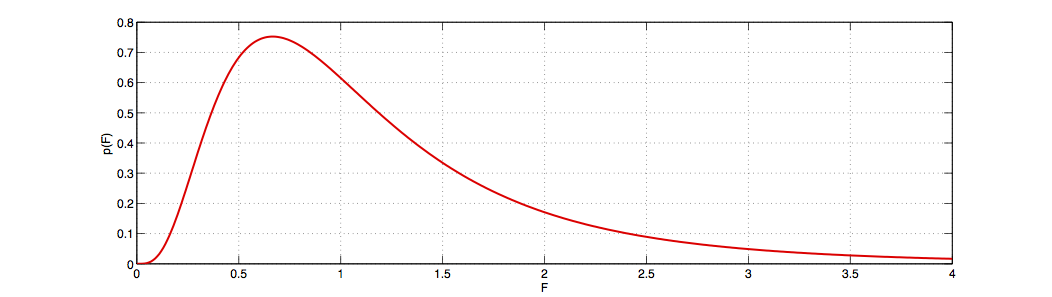
\includegraphics[width=0.8\textwidth]{fish.png}
    \end{center}
    }

    \only<2>{
    Предположения метода:
    \begin{enumerate}
    \item распределения признака во всех группах нормально;
    \item для фактора с более чем двумя уровнями: попарные разности признака имеют одинаковую дисперсию для любых уровней фактора (сферичность);
    \item объекты независимы.
    \end{enumerate}

    \bigskip

    Предположение сферичности на практике нарушается наиболее часто, причём это может привести к росту вероятности ошибки первого рода.
    }

    \only<3>{
    \begin{block}{Пример, Pearson, 2003} Исследовалось влияние метилфенидата на~способность к~отсрочке удовольствия умственно отсталыми детьми с~синдромом дефицита внимания и гиперактивности. Каждый испытуемый принимал либо препарат в одной из трёх дозировок, либо плацебо, после чего проходил тест.
    \end{block}
    \bigskip

    $H_0 \colon$ препарат не влияет на среднюю способность к отсрочке удовольствия.

    $H_1 \colon$ препарат влияет на среднюю способность к отсрочке удовольствия $\Rightarrow p = 0.004.$
    }
\end{frame}

\begin{frame}{Критерий Фридмана}
    \only<1>{
    \begin{center}
        \begin{tabular}{rl}
            выборки:                        & $X_{ki} = \mu + \alpha_k + \beta_i + \varepsilon_{ki}, \;\;i=1,\dots,n, \; k=1,\dots,K$ \\
            нулевая гипотеза:               & $H_0\colon \alpha_1=\ldots=\alpha_K$ \\
            альтернатива:                   & $H_1\colon H_0$ неверна\\
            статистика:                     & $S\left(X\right) = \frac{12}{nK\left(K+1\right)} \sum\limits_{k=1}^{K} R_k^2 - 3n\left(K-1\right)$\\
                                            & $R_k = \sum\limits_{i=1}^{n} r_{ki}$\\
                                            & $r_{ki}$~--- ранг $k$-го элемента в $i$-й строке\\
            нулевое распределение:          & табличное\\

        \end{tabular}
    \end{center}
    Распространённая аппроксимация для $n>15, K>10$:
    $$S\left(X\right) \sim \chi^2_{K-1}.$$
    Более точная аппроксимация:
    $$\frac{\left(n-1\right)S\left(X\right)}{n\left(K-1\right)-S\left(X\right)} \sim F\left(n-1, \left(n-1\right)\left(K-1\right) \right).$$
    }

    \only<2>{
    \begin{block}{Пример} Исследуется 5~технологий вытачивания детали. Каждый из~15~рабочих в течение нескольких смен использовал каждую из~технологий. $X_{ki}$~--- производительность $i$-го рабочего при использовании $k$-й~технологии.
    \end{block}
    \bigskip

    $H_0 \colon$ выбор технологии не меняет производительности рабочих.

    $H_1 \colon$ выбор технологии влияет на производительность рабочих $\Rightarrow p = 0.356.$
    }
\end{frame}

\begin{frame}{Критерий Пейджа}
    \only<1>{
    \begin{center}
        \begin{tabular}{rl}
            выборки:                        & $X_{ki} = \mu + \alpha_k + \beta_i + \varepsilon_{ki}, \;\;i=1,\dots,n, \; k=1,\dots,K$ \\
            нулевая гипотеза:               & $H_0\colon \alpha_1=\ldots=\alpha_{K}$ \\
            альтернатива:                   & $H_1\colon \alpha_1\leq\ldots\leq\alpha_{K}$\\
            статистика:                     & $L\left(X\right) = \sum\limits_{k=1}^{K} kR_k$\\
                                            & $R_k = \sum\limits_{i=1}^{n} r_{ki}$\\
                                            & $r_{ki}$~--- ранг $k$-го элемента в $i$-й строке\\
            нулевое распределение:          & табличное\\
        \end{tabular}
    \end{center}

    \bigskip

    Аппроксимация для $n>15, K>10$:
    $$ L\left(X\right) \sim N\left(\frac{nK\left(K+1\right)^2}{4}, \frac{n\left(K^3 - K\right)^2}{144\left(K-1\right)}\right).$$
    }

    \only<2>{
    \begin{block}{Пример, Лагутин, 17.3.2} На $3$ полях тестируется $5$ доз калийных удобрений. Каждое поле поделено на $5$ участков, по одному на каждую дозу. Измерена прочность выращенного на каждом участке хлопка.
	\end{block}
	\begin{center}
		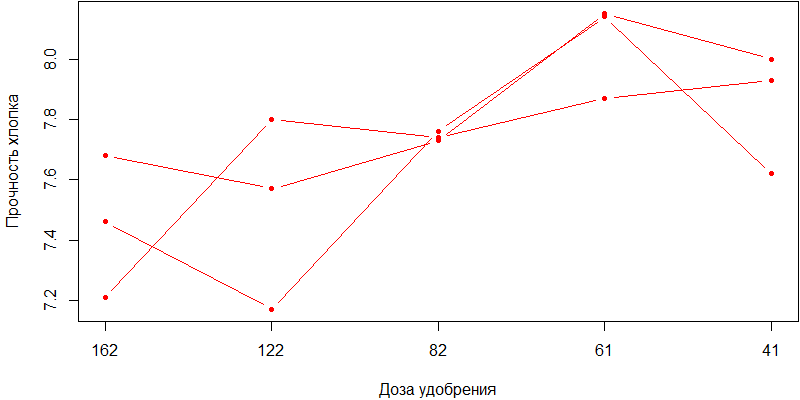
\includegraphics[width=0.65\textwidth]{cotton.png}	
	\end{center}
	
	$H_0 \colon$ дозировка удобрений не влияет на прочность хлопка.
	
	$H_1 \colon$ дозировка удобрений влияет на прочность хлопка $\Rightarrow p = 0.0663.$
	
	$H_1 \colon$ с ростом дозировки удобрений прочность хлопка уменьшается $\Rightarrow p <0.01.$
}
\end{frame}

%\begin{frame}{Пример}
%	Выведение нейролептиков у шизофреников (для самостоятельной работы):
%	
%	\url{https://yadi.sk/i/C-F91VFApY5D9}
%\end{frame}

\section{}
\begin{frame}{Литература}
    \only<1>{
    \begin{itemize}
    \item разновидности ANOVA~--- Tabachnick, 3.2;
%    \item применение в R~--- Chang, \burl{http://www.cookbook-r.com/Statistical_analysis/ANOVA/};
%    \item проверка однородности дисперсии в R: \burl{http://www.cookbook-r.com/Statistical_analysis/Homogeneity_of_variance/};
    \item unbalanced two-way ANOVA~--- Tabachnik, 6;
    \item критерии Краскела-Уоллиса (Kruskal–Wallis) и Джонкхиера (Jonckheere)~--- Кобзарь, 4.2.1.2.1, 4.2.1.2.9;
    \item критерии Фридмана (Friedman) и Пейджа (Page)~--- Лагутин, гл. 17;
    \item перестановочные аналоги~--- Bonnini, гл. 3, 4;
    \item критерий Маухли (Mauchly's sphericity test), поправки при отсутствии сферичности (Huynh-Feldt, Greenhouse-Geisser, lower-bound)~--- \url{http://en.wikipedia.org/wiki/Mauchly's_sphericity_test};    
    \item profile analysis~--- альтернатива w.s. ANOVA~--- Davis;
	\item \textbf{примеры проведения дисперсионного анализа в R:}
	
		\href{http://www.uni-kiel.de/psychologie/rexrepos/posts/anovaCRp.html}{1-way b.s.},
	    \href{http://www.uni-kiel.de/psychologie/rexrepos/posts/anovaCRFpq.html}{2-way b.s.},
	    \href{http://www.uni-kiel.de/psychologie/rexrepos/posts/anovaRBp.html}{1-way w.s.},
	    \href{http://www.uni-kiel.de/psychologie/rexrepos/posts/anovaRBFpq.html}{2-way w.s.}
    \end{itemize}
	}
	
	\only<2>{
	
    {\small
     Лагутин М.Б. \textit{Наглядная математическая статистика}, 2007.
		
		\vspace{5pt}
		
     Кобзарь А.И. \textit{Прикладная математическая статистика}, 2006.     
		
		\vspace{5pt}
		
     Beall G. (1942). \textit{The Transformation of data from entomological field experiments}. Biometrika, 29, 243–262.
		
		\vspace{5pt}
		
	 Bonnini S., Corain L., Marozzi M., Salmaso S. \textit{Nonparametric Hypothesis Testing - Rank and Permutation Methods with Applications in R}, 2014.     
		
		\vspace{5pt}
		
     Davis C.S. \textit{Statistical Methods for the Analysis of Repeated Measurements}, 2002.
		
		\vspace{5pt}
			
	 Pagano R.R. \textit{Understanding Statistics in the Behavioral Sciences}, 2012.
		
		\vspace{5pt}
	
     Pearson D.A, Santos C.W., Roache J. D., et al. (2003). \textit{Treatment effects of methylphenidate on behavioral adjustment in children with mental retardation and ADHD}. Journal of the American Academy of Child and Adolescent Psychiatry, 42(3), 209-216. 
		
		\vspace{5pt}
		
     Tabachnick B.G., Fidell L.S. \textit{Using Multivariate Statistics}, 2012.
    }
	}
\end{frame}
\end{document}
